%\part{Konstruktion}
%\chapter{Programmlogik}

\section{SEARCHExtraction}
Die SearchExtraction nimmt ein \lstinline|WebContent|-Objekt entgegen und verarbeitet es zu einem \lstinline|SearchModels|-Objekt. Hierbei wird der HTML-Code, der im \lstinline|WebContent| enthalten ist, auf Search-Tags abgesucht. Diese Search-Tags werden dann zu \lstinline|SearchModel|-Objekten zusammengebaut und in einem \lstinline|SearchModels|-Objekt gesammelt.\newline
Für den Ablauf der Analyse und Erzeugung ist der \lstinline|SearchManager| zuständig. Die Methoden für die Analyse des HTML-Codes stellt die \lstinline|RegexForSEARCH| zur Verfügung.

\begin{figure}[h]
	\centering
	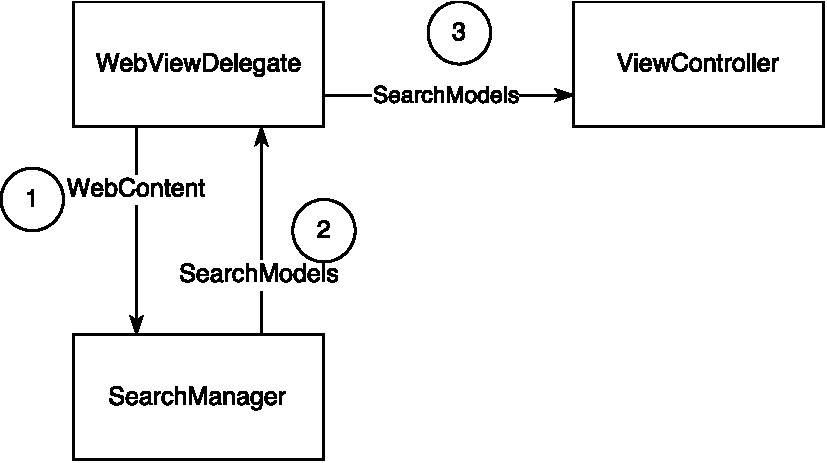
\includegraphics[width=\textwidth]{UI_WebContent_SearchModel_Usage}
	\caption{Umwandeln eines WebContent-Objekts in ein SearchModels-Objekt}
	\label{fig:WebContent zu SearchModels}
\end{figure}

Die obige Darstellung beschreibt den Ablauf und die Übergabestellen der Schnittstellen \lstinline|WebContent| und \lstinline|SearchModels|. Der \lstinline|WebContent|, erzeugt vom \lstinline|WebViewDelegate|, wird in Schritt 1 dem \lstinline|SearchManager| übergeben. Der \lstinline|SearchManager| erzeugt aus dem \lstinline|WebContent| die \lstinline|SearchModels| und gibt diese in Schritt 2 an den \lstinline|WebViewDelegate| zurück. Der \lstinline|WebViewDelegate| übergibt dann das \lstinline|SearchModels|-Objekt an den \lstinline|ViewController|, wo es zur Verfügung für die anderen Packages steht.

\subsection{SearchManager}
\subsection{RegexForSEARCH}

%\subsubsection{Unterteilabschnitt}
%\paragraph{Paragraph}
%\subparagraph{Unterparagraph}
